\documentclass[border=10pt]{standalone}

\usepackage{tikz}
\usepackage{tikzsymbols}
\usetikzlibrary{calc,patterns,shapes.geometric}

\def\centerarc[#1](#2)(#3:#4:#5){\draw[#1] ($(#2)+({#5*cos(#3)},{#5*sin(#3)})$) arc (#3:#4:#5);}

\begin{document}
	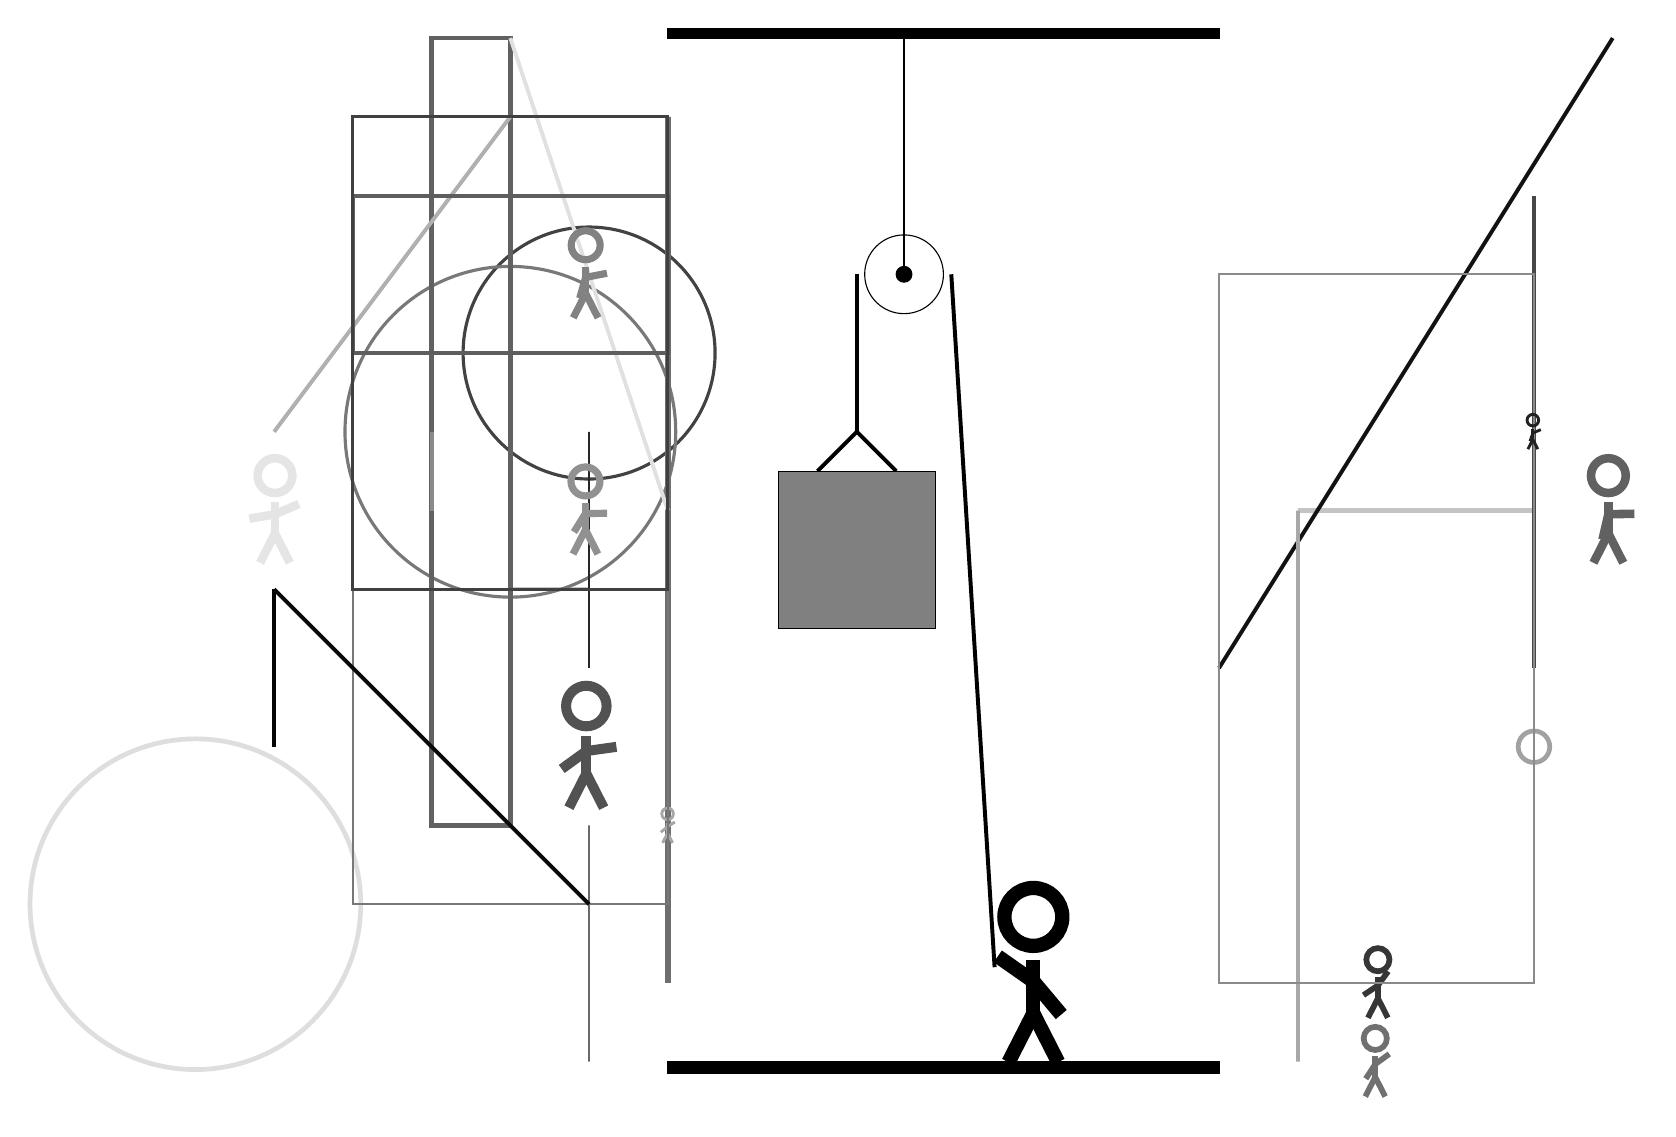
\begin{tikzpicture}
		%%%%% START %%%%%
		
		\draw[fill=black] (-2, 10) rectangle (5, 10.125);
		
		\draw (1, 7) circle (0.5);
		\draw[fill=black] (1, 7) circle (0.1);
		\draw (1, 10) -- (1, 7);
		
		\draw[line width=0.5mm] (-0.1, 4.5) -- (0.4, 5.0) -- (0.9, 4.5);
		\draw[fill=black!50] (-0.6, 4.5) rectangle (1.4, 2.5);
		
		\draw[line width=0.5mm] (0.4, 7) -- (0.4, 5.0);
		\centerarc[line width=0.5mm](1, 7)(0:180:0.6);
		\draw[line width=0.5mm](1.6, 7) -- (2.15, -1.8);
		
		\draw[line width=0.5mm, color=black!22] (-4, 3) rectangle (-3, 3);
		
		\draw[line width=0.6mm, color=black!23] (6, 4) rectangle (9, 4);
		\draw [line width=0.4mm, color=black!74](-3, 6) circle (1.6);
		\draw [line width=0.4mm, color=black!53](-4, 5) circle (2.1);
		
		\draw[line width=0.6mm, color=black!62] (-4, 10) rectangle (-5, 0);
		
		\draw[line width=0.5mm, color=black!93](10, 10) -- (5, 2);
		\draw[line width=0.5mm, color=black!31](-7, 5) -- (-4, 9);
		
		\draw[line width=0.7mm, color=black!57] (-2, -2) rectangle (-2, 9);
		\draw[line width=0.3mm, color=black!59] (-3, -3) rectangle (-3, 0);
		\draw [line width=0.6mm, color=black!37](9, 1) circle (0.2);
		\draw[line width=0.5mm, color=black!12](-2, 4) -- (-4, 10);
		\node[line width=0.7mm, color=black!35] at (-2, 0) {\Strichmaxerl[2][39][33]};
		\node[line width=0.5mm, color=black!49] at (-3, 7) {\Strichmaxerl[5][74][11]};
		
		\draw[line width=0.5mm, color=black!72](9, 8) -- (9, 2);
		\draw [line width=0.6mm, color=black!13](-8, -1) circle (2.1);
		\draw[line width=0.5mm, color=black!34] (6, -3) rectangle (6, 4);
		
		\draw[line width=0.2mm, color=black!85] (-3, 5) rectangle (-3, 2);
		
		\draw[line width=0.2mm, color=black!53] (-2, 9) rectangle (-6, -1);
		\node[line width=0.6mm, color=black!79] at (7, -2) {\Strichmaxerl[4][34][54]};
		\node[line width=0.5mm, color=black!62] at (10, 4) {\Strichmaxerl[6][77][1]};
		\node[line width=0.4mm, color=black!68] at (-3, 1) {\Strichmaxerl[7][36][8]};
		
		\draw[line width=0.5mm, color=black!98](-7, 1) -- (-7, 3);
		\draw[line width=0.2mm, color=black!46] (5, -2) rectangle (9, 7);
		\node[line width=0.7mm, color=black!56] at (7, -3) {\Strichmaxerl[4][57][36]};
		\node[line width=0.3mm, color=black!43] at (-3, 4) {\Strichmaxerl[5][58][1]};
		
		\node[line width=0.2mm, color=black!87] at (9, 5) {\Strichmaxerl[2][71][23]};
		\draw[line width=0.5mm, color=black!96](-7, 3) -- (-3, -1);
		\draw[line width=0.5mm, color=black!63] (-2, 6) rectangle (-6, 8);
		\draw[line width=0.5mm, color=black!46](-5, 5) -- (-5, 4);
		
		\draw[line width=0.4mm, color=black!75] (-2, 9) rectangle (-6, 3);
		\node[line width=0.2mm, color=black!10] at (-7, 4) {\Strichmaxerl[6][10][23]};
		
		
		\node at (2.6, -1.9) {\Strichmaxerl[10][-35][-50]};
		
		\draw[fill=black] (-2, -3) rectangle (5, -3.15);
		
		%%%%% END %%%%%
	\end{tikzpicture}
\end{document}